\documentclass{article}
\usepackage[utf8]{inputenc}
\usepackage{graphicx}
\usepackage{booktabs}
\usepackage{siunitx}
\usepackage{caption}
\begin{document}
\section*{So sánh nghiệm analytic và nghiệm số (1D bar)}
\begin{figure}[ht]
  \centering
  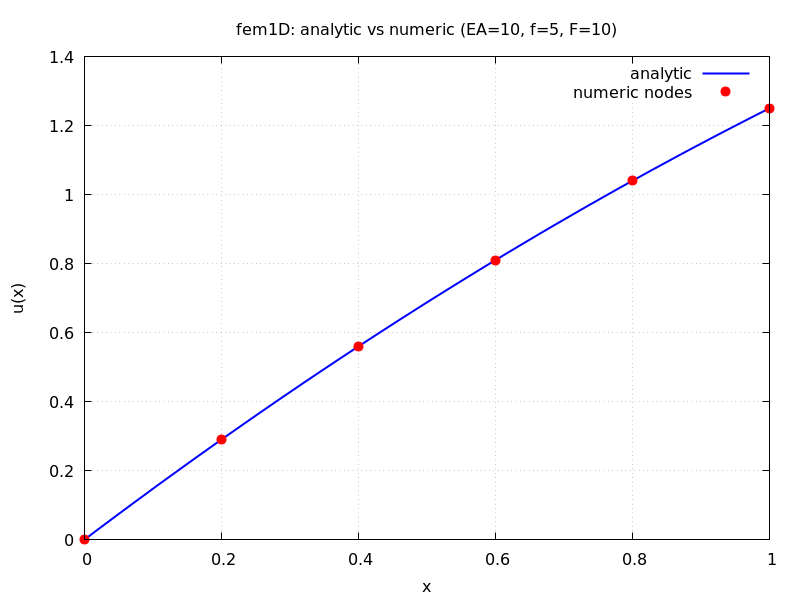
\includegraphics[width=0.9\linewidth]{fem1D_compare.png}
  \caption{So sánh nghiệm analytic và các điểm nút nghiệm số (EA=10, $f=5$, $F=10$).}
\end{figure}

\vspace{1em}
\begin{table}[ht]
  \centering
  \sisetup{round-mode=places,round-precision=2}
  \begin{tabular}{c S S}
    \toprule
    $x$ & {$u_{analytic}$} & {$u_{numeric}$} \\
    \midrule
    0.0 & 0.00 & 0.00 \\
    0.2 & 0.29 & 0.29 \\
    0.4 & 0.56 & 0.56 \\
    0.6 & 0.81 & 0.81 \\
    0.8 & 1.04 & 1.04 \\
    1.0 & 1.25 & 1.25 \\
    \bottomrule
  \end{tabular}
  \caption{Giá trị nghiệm analytic và nghiệm số tại các nút (lưới 5 phần tử).}
\end{table}

\end{document}
